\section{Evaluation}
\subsection{Evaluation of the application}
\subsection{Evaluation of the models}
To evaluate our model, we have decided to model the paediatric pneumonia guideline \parencite{RepublicofKeny2016}. As we have a strict time limitation it is better for us to evaluate a respiratory condition, as we have already worked with a respiratory condition in asthma. There is quite a lot of work for software developers to learn a new clinical guideline, so we save a lot of time when the concepts are similar.

In figure \ref{fig:PneumoniaEntityGraph} we have modelled the entity model of the paediatric pneumonia guideline \parencite{RepublicofKeny2016}. We see that both guidelines have a history part, where the patient or dependants can tell something about the condition of the patient. Both guidelines also have an examination part where the clinician looks for several symptoms. The symptoms are a bit different from paediatric possible asthma guideline, but they have several symptoms in common. Wheeze is something the clinician has to be aware about. If the patient is wheezing, the patient should be treated according to the paediatric possible asthma guideline instead.

The management part is also quite similar to the paediatric possible asthma guideline. The patient and dependants will be given some advise concerning the medical condition of the patient. If the pneumonia is severe, or the patient has lower chest wall indrawing and the patient cannot be reviewed within 48 hours, the patient should be admitted into the hospital. The medication is quite similar to the paediatric possible asthma guideline. For pneumonia there are fewer medications, but both guidelines have treatment with antibiotics and oxygen.

The big difference is the diagnostic part. For the paediatric possible asthma guideline, there is only one medical condition described. However, for the paediatric pneumonia guideline patients with tuberculosis or HIV will receive a different treatment. We have not modelled the treatment for pneumonia patients with HIV or tuberculosis as they are separate guidelines. But we need to identify such patients and refer to their respective guidelines. The same goes for asthma. Wheezing patients needs to be identified for asthma treatment.

To support several conditions, we have used inheritance on the diagnosis vertex. A new problem occurs as how should we model tuberculosis, no tuberculosis and that we don't know if the patient has tuberculosis? Earlier on, we used the open world principle for the symptoms. If the vertex doesn't exist, we haven't done the examination for the symptom and we don't know if the patient has it or not. The same goes for diagnosis. If the vertex is not there, we need to clarify if the patient has tuberculosis. To model the situation where we know that the patient hasn't tuberculosis, we have introduced the diagnosis "no tuberculosis". An alternative solution could be to introduce an attribute "status". The attribute could hold information about the patient evidently has the condition, evidently don't have the condition and if it is not clarified. A fourth status could be if the condition is recurring.

\begin{figure}[h!]
	\label{fig:PneumoniaEntityGraph}
	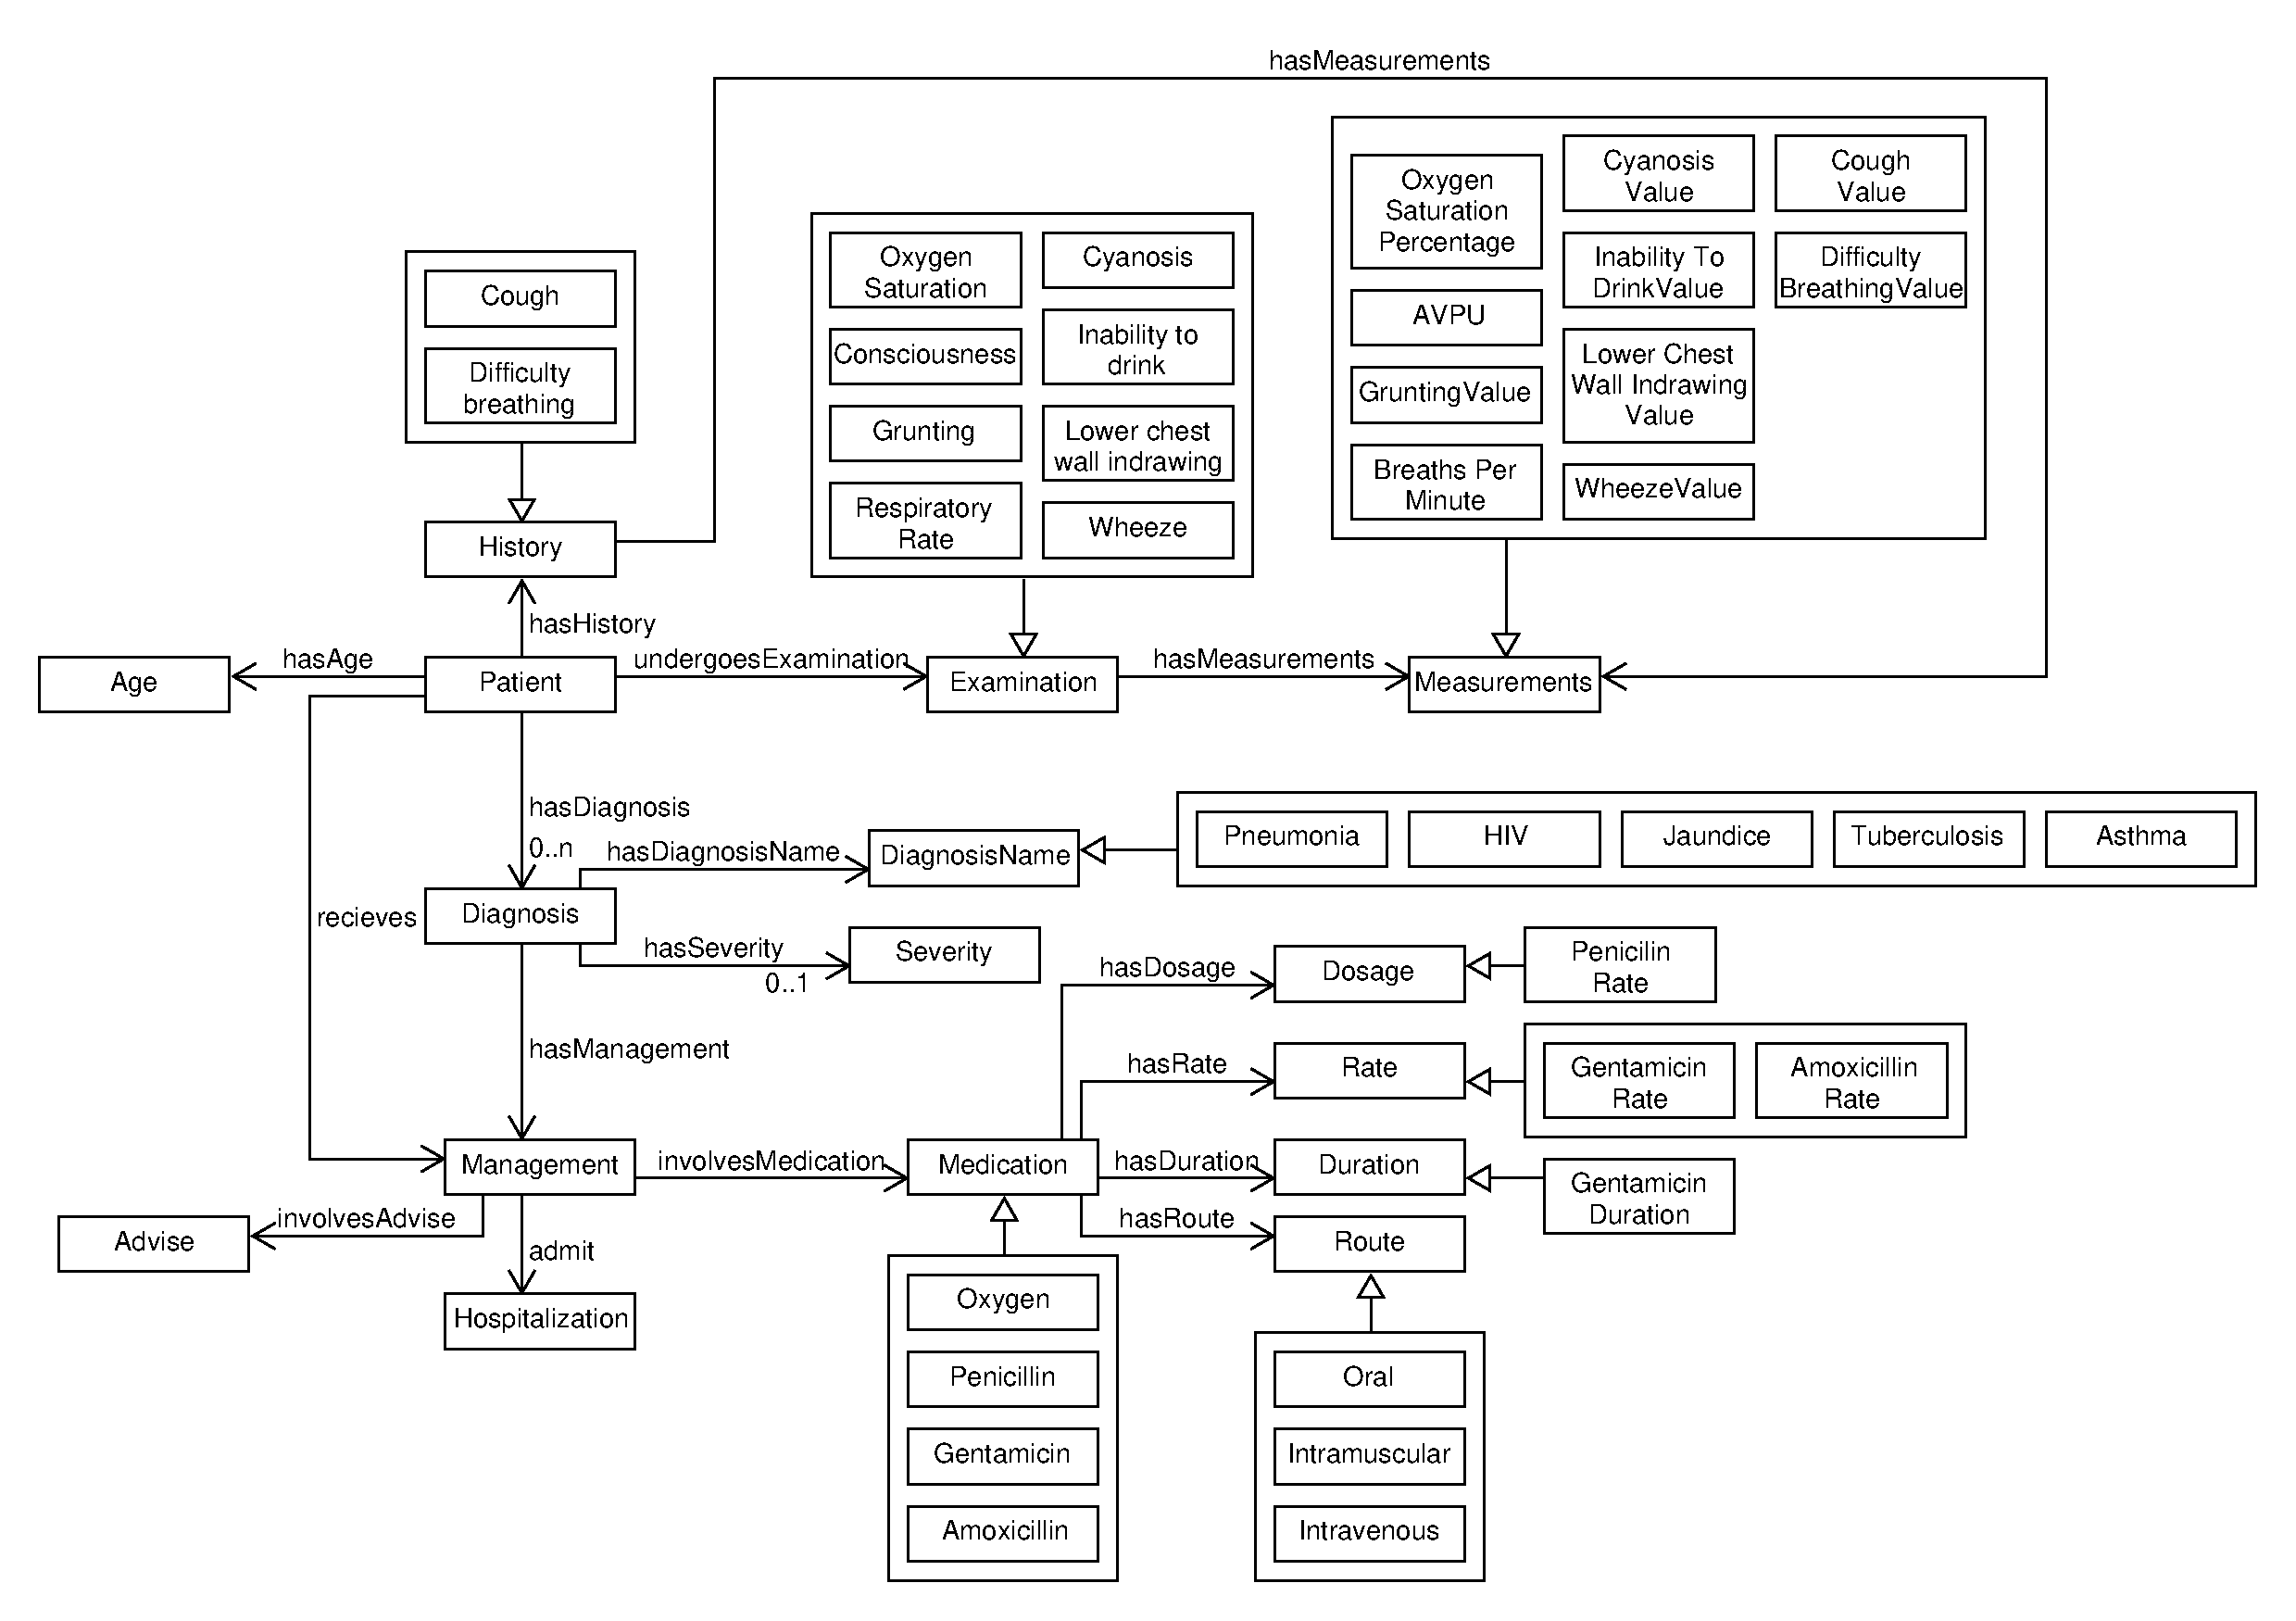
\includegraphics[scale=0.33]{PneumoniaEntityGraph}
	\caption {We are showing that our model is general enough to represent other CPGs. Here we have modelled the paediatric pneumonia guideline \parencite{RepublicofKeny2016}}
\end{figure}

To evaluate the workflow model in figure \ref{fig:WorkflowGraph}, we do like we did for the paediatric possible asthma guideline \parencite{RepublicofKeny2016}. We see the guideline in combination with the entity entity and the workflow model. The paediatric possible asthma guideline \parencite{RepublicofKeny2016} has an assessment part, where we look for patient older than 60 days, cough or difficulty breathing. If he has those symptoms and does not wheeze, we continue looking for other pneumonia symptoms. In the diagnostic part we strengthen our assumption of pneumonia, we set the severity of the diagnosis and we further keep in mind that if the the patient is wheezing he should be given the asthma treatment. Pneumonia patients with HIV or tuberculosis should be referred to specific guidelines for those condition combinations \parencite{RepublicofKeny2016}. In the management part, some patients get admitted into the hospital. The management further has an advise for review within 48 hours. The patients condition is then evaluated either on the hospital for admitted patients, or in a review within 48 hours for other patients. We can conclude with that the workflow model  also covers the paediatric pneumonia guideline \parencite{RepublicofKeny2016}.

In figure \ref{fig:PneumoniaPneumoniaIntegratedEntityWorkflowModels} we demonstrate an instance of the entity model working together with an instance of the workflow model. The patient goes through assessment, diagnosis, management and evaluation. As the patient has jaundice, he won't receive penicillin treatment. As the the pneumonia is severe, the treatment will be evaluated at the hospital and schedule for review is unnecessary. 
\begin{figure}[h!]
	\label{fig:PneumoniaPneumoniaIntegratedEntityWorkflowModels}
	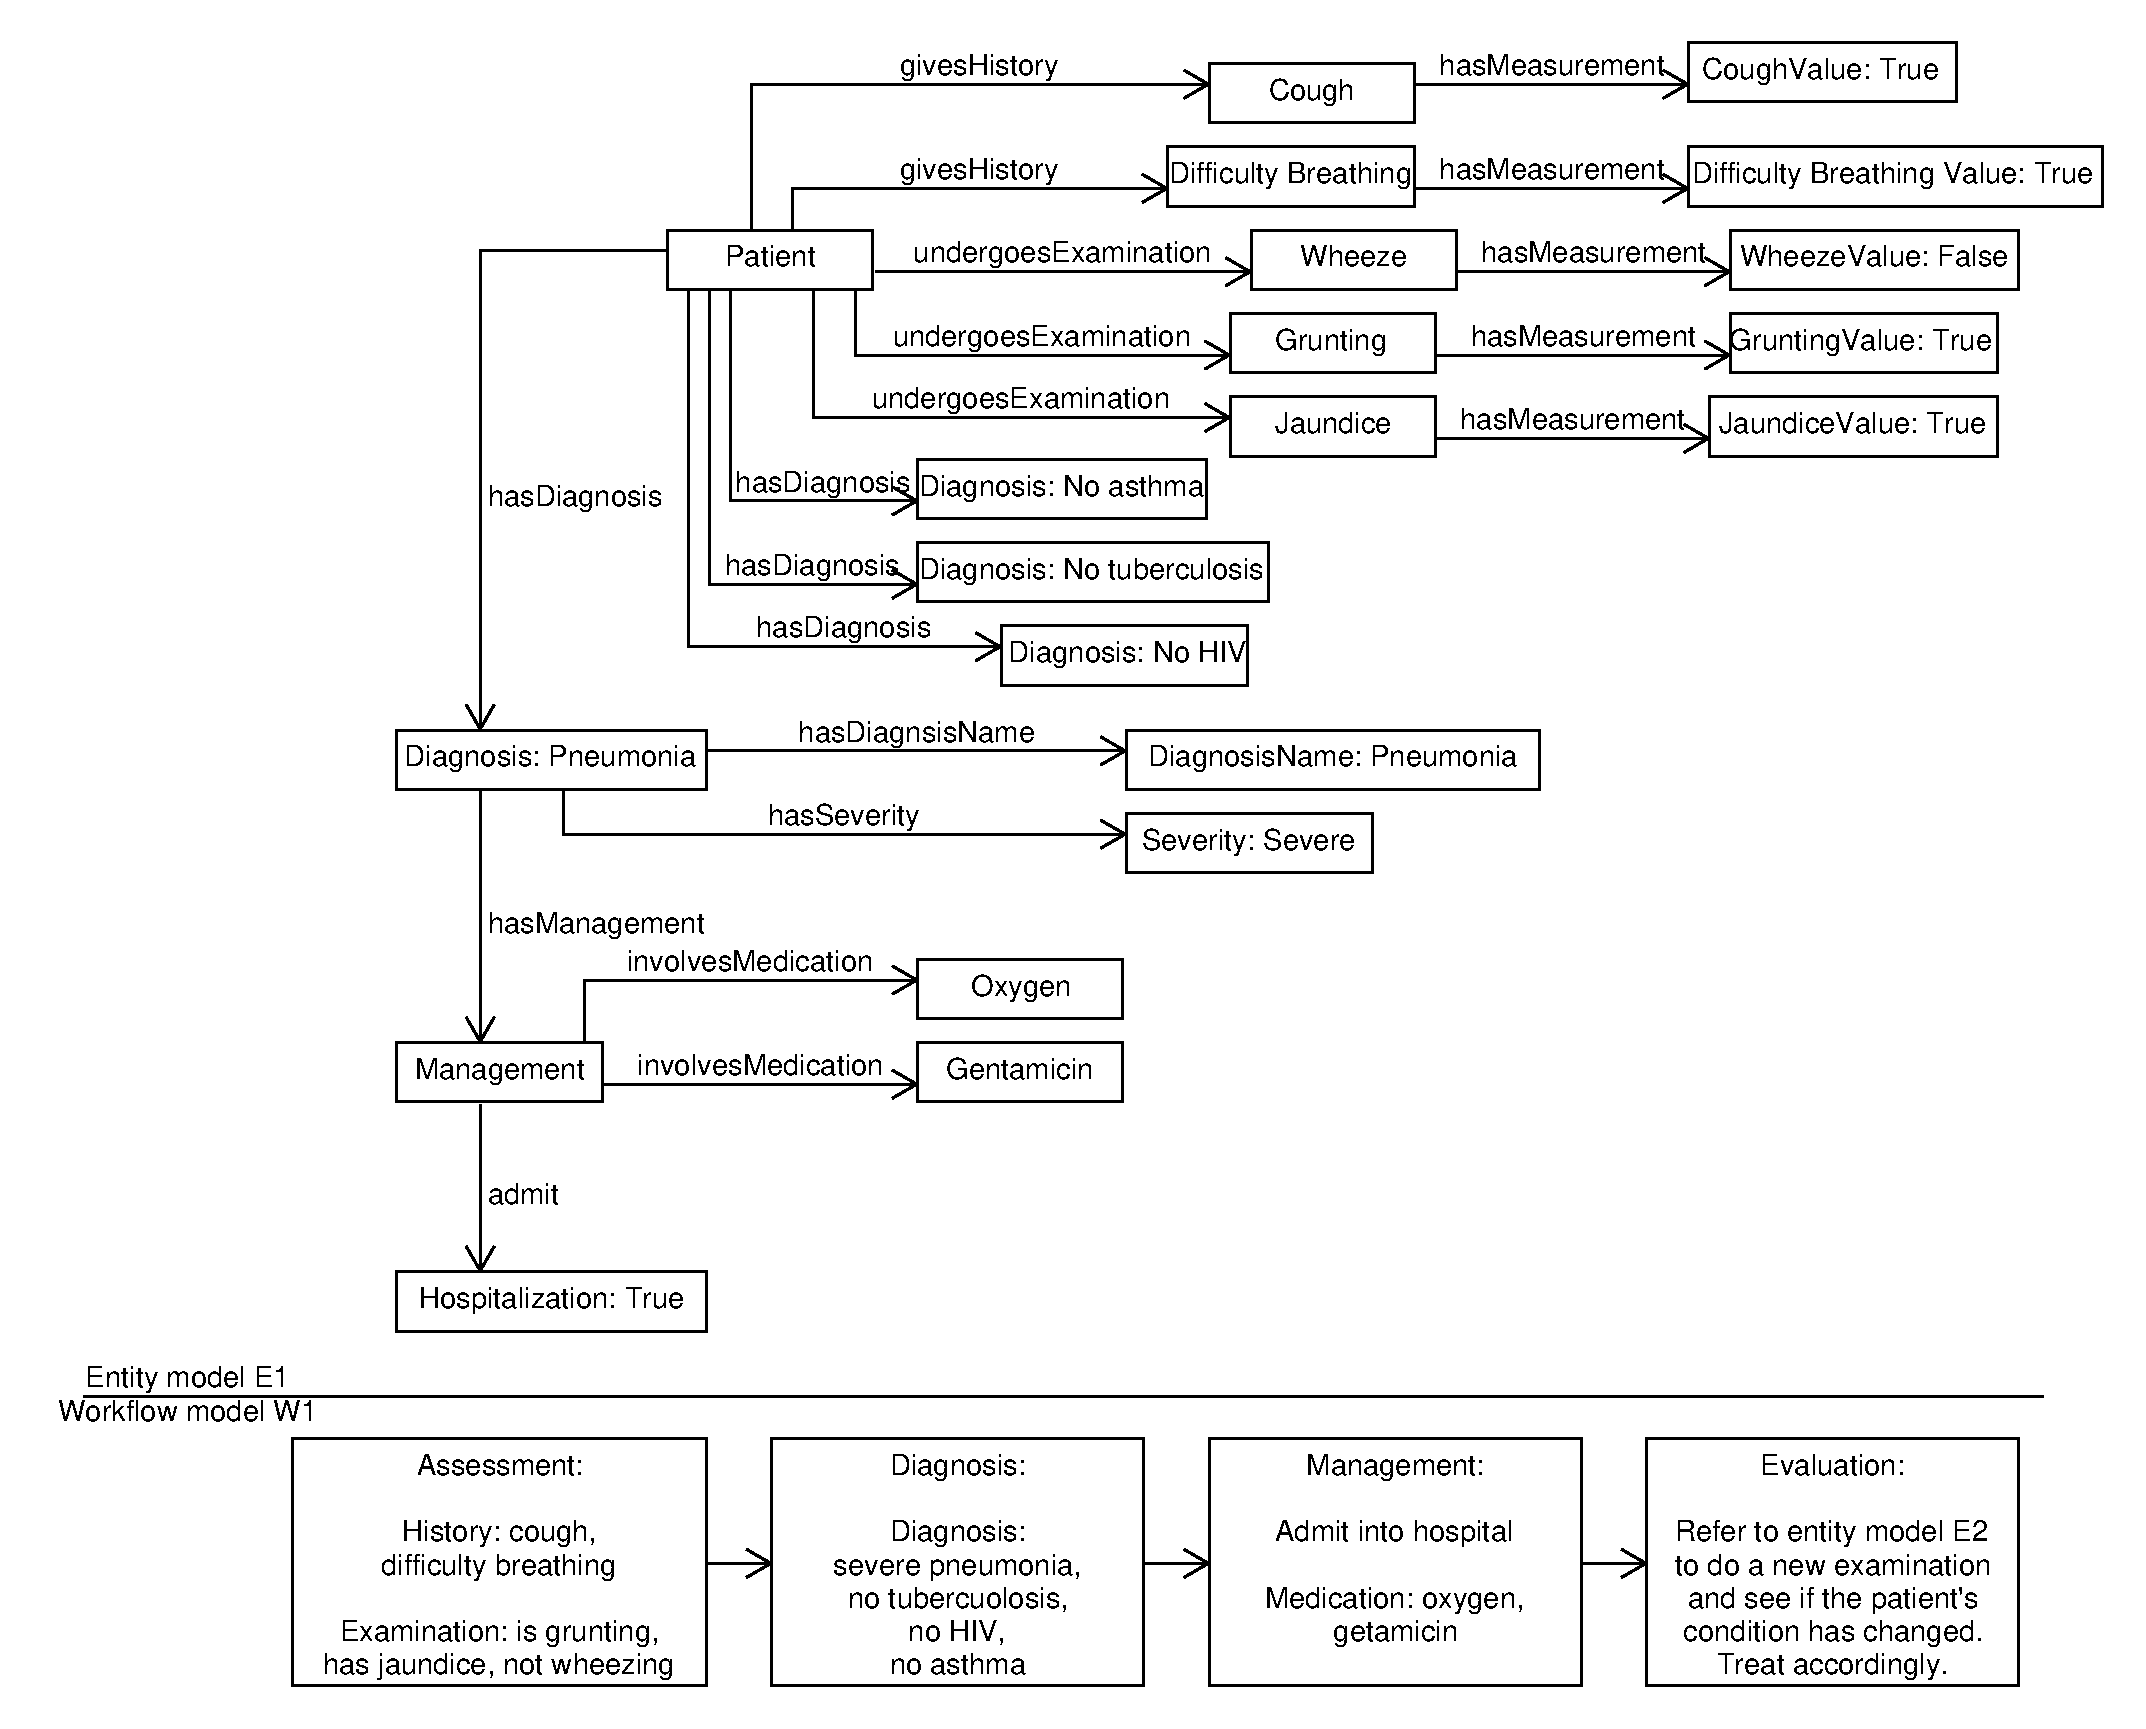
\includegraphics[scale=0.4]{PneumoniaIntegratedEntityWorkflowModels}
	\caption {We are showing out entity model working together with the workflow model for paediatric pneumonia guideline \parencite{RepublicofKeny2016}}	
\end{figure}

After the evaluation, we see that we have modified the entity and workflow models to support both pneumonia and asthma in paediatric medicine. It is likely that further modification and expansion of the entity model is needed when modelling other CPGs. However, we see that we have identified reusable elements of the guidelines, and our models can work as a stepping stone for guideline formalization standardisation.
\section{Limitations of the model}
\begin{itemize}
	\item Can't ask questions like "what are the symptoms for severe asthma?"
	\item Difficult to ask what NOT to do. If the vertex doesn't exist, only an empty string gets returned. Can only be used were we actually have written "don't admit to the hospital" as an example with hospitalization.
	\item \textcolor{purple}{TODO Yngve: Graph QL?}The inheritance makes it difficult to generalize some questions. We can't make a template which asks about the Rate a medicine should be taken with. We need to specifically ask for that medicine. To be able to ask for a general medicine, one solution can be to introduce a new tag which compares the substring of the type of the vertex. Another solution is to use the meta model and not the instance model. We don't use inheritance on diagnosis because of this.
	\item To avoid the problem described in the previous point, we don't use inheritance on Diagnosis. A limitation here is that  
	a patient can only have one diagnosis.
\end{itemize}